 \documentclass{article}
 \usepackage{graphicx}
 \graphicspath{ {./images/} }
 
 \usepackage{hyperref}
 \hypersetup{
    colorlinks=true,
    linkcolor=blue,
    filecolor=magenta,      
    urlcolor=cyan,
 }

 \usepackage{parskip}
 \usepackage{amsmath}
 
 \begin{document}
 
 \begin{center}
     \Huge\textbf{Homework 4: Sukrit Ganesh}\par
 \end{center}
 
  \noindent\makebox[\linewidth]{\rule{\paperwidth}{0.4pt}}\newline
 
 \begin{center}
      \Large\textbf{Exercise 1: }Propose a family of learning rates that satisfies assumption 4 (a formal proof is not needed).\par
 \end{center}
 
 We must find learning rates which satisfy the following assumption:  In other words, the sum of the learning rates is unbounded, but the sum of their
 squares is bounded.
 
 \[\sum_{n=1}^{\infty}{\eta}_{n}=\infty\]
 \[\sum_{n=1}^{\infty}{\eta}_{n}^2=c\]

 We need to find a sequence whose series is divergent but whose sum of squares form a convergent series. The harmonic series $\sum_{n=1}^{\infty}\frac{1}{n}$ is divergent, but the squared harmonic series $\sum_{n=1}^{\infty}\frac{1}{n^2}$ is convergent. Thus, our learning rates can be the harmonic sequence.
 
 However, there are more sequences which fit our definition. In fact, we can try finding any series $\sum^{n=1}_{\infty}n^{\alpha}$ which diverges, but converges when we square the terms (in other words, multiply $\alpha$, the exponent, by 2). In this case, we want $\alphs$ to be between -1 and -0.5. In order to converge, $\alpha$ must be above -1, but we also want $2*\alpha$ to be less than -1 so that the squared series diverges. Therefore, we want $\alpha$ to be greater than -1 and less than -0.5.
 
 We can express the family of learning rates as follows: $1^{\alpha}, 2^{\alpha}, 3^{\alpha}, ...$, where $-1 \leq \alpha \leq -0.5$.
 
 \newpage
 
 \noindent\makebox[\linewidth]{\rule{\paperwidth}{0.4pt}}\newline
 
 \begin{center}
      \Large\textbf{Exercise 2:} \par
 \end{center}
 
 \textbf{Part 1: | }Prove the following relationship for any two random variables $u, v$: $E_u[f(u)]=E_v[E_{u|v}[f(u)|v]]$.\newline
 
 Let $m = f(u)$. We need to prove the following:
 
 \[E[m] = E_v[E_{m|v}[m|v]]\]
 
 We will express our expected value as an integral for the purposes of our proof.
 
 \[E[m] = \int_{-n}^{n}mf(m)dm\]
 
 We will use marginal probability density function.

 \[E[m]=\int_{-n}^{n}f(v|m)dv\]
 
 \[E[m]=\int_{-n}^{n}m\int_{-n}^{n}f(m|v)f(v)dvdm\]
 
 \[E[m]=\int_{-n}^{n}\Bigg[\int_{-n}^{n}mf(m|v)dm\Bigg]f(v)dv\]
 
 \[E[m]=\int_{-n}^{n}\Bigg[E[m|v]\Bigg]f(v)dv\]
 
 \[E[m]=E\big[E[m|v]\big]\]
 
 \[E[m]=E\big[E[f(u)|v]\big]\]
 
 \textbf{Part 2: | }Knowing that noise is bounded, show that $E[y_n^2]$ is also bounded.\newline
 
 We know that $P(|y|< c)=1$ where $c \geq 0$. In other words, the noise is bounded between $\pm c$.
 
 This also applies to the squared noise: $P(y^2 < c^2)=1$ where $c \geq 0$. We see that the squared noise is bounded between $\pm c^2$.
 
 We can use Markov inequality.
 
 \[P(y^2\geq c^2)\leq\frac{E[y^2]}{c^2}\]
 
 This implies the following.
 
 \[P(y^2\leq c^2)\geq\frac{E[y^2]}{c^2}\]
 
 We see that $E[y]$ is bounded, so $E[y^2]$ is also bounded.\newline
 
 \textbf{Part 3: | }Given that $E[y_n^2]$ is bounded, show that  $\sum_{i=1}^{n}{{\eta}_i}^2E[y_n^2]$.\newline
 
 Markov's inequality from part 2 states the following: $P(y^2\leq c^2)\geq\frac{E[y^2]}{c^2}$. We can rearrange the terms to get the following: $P(y^2\leq c^2)c^2\geq E[y^2]$. This shows that the upper bound of $E[y^2]$ is $c^2$, because $P(y^2\leq c^2) \leq 1$.
 
 We already know that $\sum_{i=1}^{n}{n_i}^2$ is bounded at some value $d$. Because $E[y_n^2]$ is at most $c^2$, $\sum_{i=1}^{n}{n_i}^2E[y_n^2]$ is bounded by value $c^2d$.\newline
 
 \textbf{Part 4: | }Prove the following: $\lim_{n \to \infty}e_n^2=0$.\newline
 
 We are given that $e_n^2$ converges. By definition, the limit of a sequence or function whose series is convergent goes to 0 on the positive infinite limit. For any $n$, ${e^2}_{n+1} < e_n^2$. Therefore, as $n$ approaches $\infty$, ${e^2}_{n+1}$ approaches 0.
 
 \newpage

 \begin{center}
      \Large\textbf{Problem 3:} Recall that root finding algorithms find the value of $x$ where a function $h(x) = 0$, and that a gradient descent algorithm finds the minimum of a function. Are these algorithms accomplishing the same goal? Briefly explain why or why not. Your answer should be limited to three lines.\par
 \end{center}
 
 They do not exactly accomplish the same goal, but they accomplish very similar goals. Ultimately, the gradient descent algorithm aims to find the minimum value (aka global minima) of a function (the derivative of the function at this point is equal to 0), whereas the root finding algorithm finds where the value of a function (not its derivative) is equal to 0. However, using the root finding algorithm on a function's derivative gives us all the local and global extrema; plugging these points into the original function can allow us to find a function's global minima.

 \newpage
 
 \begin{center}
      \Large\textbf{Exercise 4: }Do stochastic gradient descent and stochastic approximation (from section 1) accomplish the same goal? Briefly explain why or why not. Your answer should be limited to three lines.\par
 \end{center}
 
 No, they do not achieve the same goal. Stochastic gradient descent aims to minimize the error by finding the global minimum of the loss function, while stochastic approximation finds the root of a function. It is possible to use stochastic approximation to find the roots of the loss function, but this can get tricky if the loss function has multiple extrema.
 
 \newpage
 
 \begin{center}
     \Large\textbf{Exercise 5: }\par
 \end{center}
 
 We are given that $f(x)=\frac{1}{k}\sum^{j=1}_{k}Q_j(x)$.
 
 It is not difficult to prove 2.1. We know that that $g(x)=Q_i(x)$, so $E[g(x)]=E[Q(x)]$. By definition, $E[Q(x)]$ is the sum of products of probabilities of each sample (they're all of equal probability) by that sample's loss function, $Q_i(x)$. In other words, $E[Q(x)]$ is simply the average value of $Q_i(x)$ across all data points, which also happens to be the definition of $f(x)$.
 
 \textbf{Part A: | How many tickets should the airline sell to ensure that the expected number of passengers that turn up is greater than 10?}\newline
 
 The probability that n passengers will turn up can be calculated using the binomial probability formula because every passenger has an equal probability of showing up. The binomial probability formula can be written as follows:
 
 \begin{displaymath}
    P(x)={n \choose x}p^x(1-p)^{n-x}
 \end{displaymath}
 
 In the above formula, n is the number of trials, x is the number of successful trials desired, and p is the probability that a trial is successful. We can treat each ticket sold as a trial. The trial is successful if the passenger shows up, and unsuccessful if he/she decides to ditch the flight (because who wants to fly on a plane piloted by an SJW)? Ten passengers showing up (aka successes) are desired.
 
 However, we are not trying to calculate the probability that n passengers show up. Instead, we want to calculate n given the fact that 10 passengers must show up. We are simply interested in calculating n given the the expected value is 10; in other words, we want to calculate the number of tickets the airline should sell such that expected number of passengers who show up to be greater than 10. Because the number of passengers who show up is a binomial distribution, we can simply use the formula $E[x]=np$ to calculate the expected number of passengers who show up given $n$ tickets sold and $p$ being the probability that a passenger who buys a ticket shows up. The formula can be derived by finding the expected value of the binomial probability formula written above. Because we want $E[x]$ to be greater than 10, and we already know $p$, we can solve for $n$ using the following formula: $np>10$.
 
 \begin{displaymath}
    np > 10
 \end{displaymath}
 
 \begin{displaymath}
    n > \frac{10}{p}
 \end{displaymath}
 
 Final answer: $n>\frac{10}{p}$\newline
 
 \textbf{Part B: | The airline sells 10 tickets. What is the expected number of passengers on the aircraft, given that it flies? (i.e. that at least two women turn up). Estimate this value with a simulation.}\newline
 
 We used a simulation to get the following graph. We used a numpy seed of 13.\newline
 
 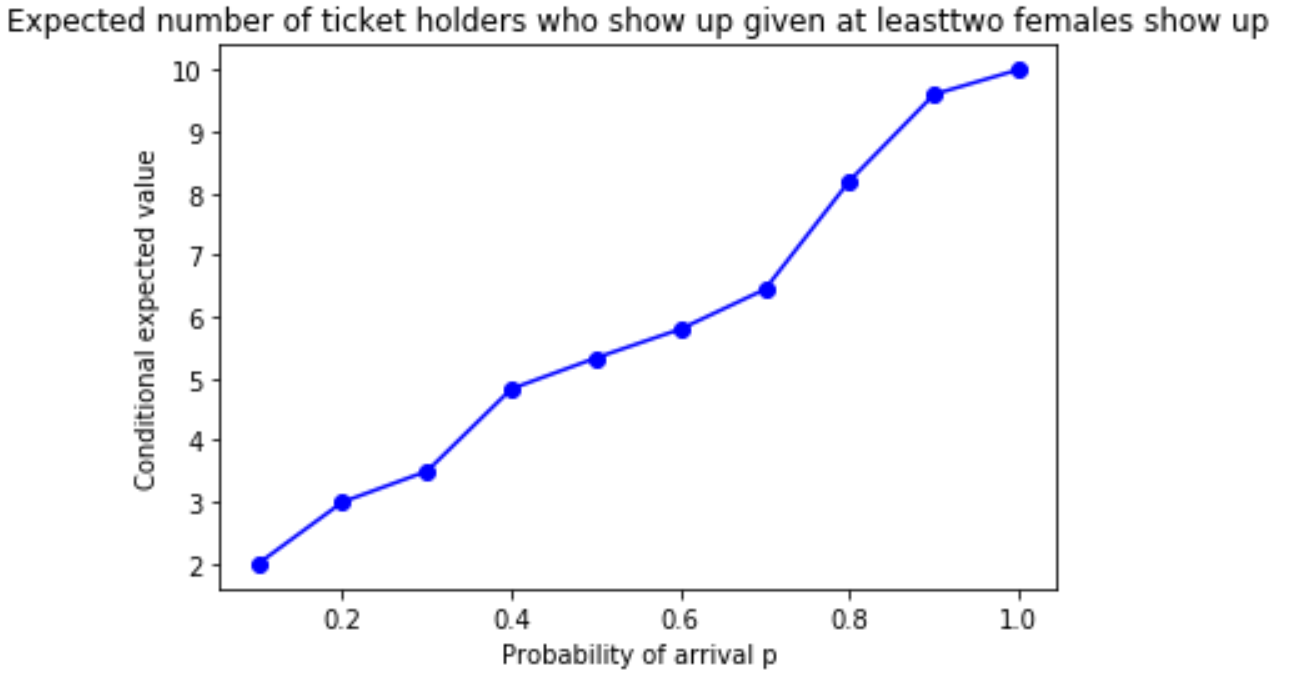
\includegraphics{HW4_5.PNG}
 
 The simulation code is attached to the end of this pdf.\newline
 
 \newpage
 
 \begin{center}
     \Large\textbf{Problem 6:} Show that if X and Y are independent random variables, then $var[X+Y] = var[X] + var[Y]$. You will find it helpful to remember that, for X and Y independent, $E[XY] = E[X]E[Y]$.\par
 \end{center}
 
 \begin{equation}
    var[X+Y] = var[X] + var[Y] + 2*cov(X,Y)
 \end{equation}
 
 The formula for co-variance of two random variables is as follows: $cov(X,Y)=E[XY]-E[X]E[Y]$. We can substitute it into our equation.
 
 \begin{equation}
    var[X+Y] = var[X] + var[Y] + 2*(E[XY]-E[X]E[Y])
 \end{equation}
 
 However, because X and Y are independent, $E[XY]=E[X]E[Y]$. We 
 
 \begin{equation}
    var[X+Y] = var[X] + var[Y] + 2*(E[X]E[Y]-E[X]E[Y])
 \end{equation}
 
 \begin{equation}
    var[X+Y] = var[X] + var[Y] + 2*0
 \end{equation}
 
 \begin{equation}
    var[X+Y] = var[X] + var[Y]
 \end{equation}
 
 Hence, we prove that when X and Y are independent random variables, $var[X+Y]=var[X]+var[Y]$.
 
 \begin{center}
      \Large\textbf{Q.E.D. :)}
 \end{center}
 
 \end{document}

